% --- Template for thesis / report with tktltiki2 class ---
% 
% last updated 2013/02/15 for tkltiki2 v1.02

\documentclass[finnish]{tktltiki2}
\nonstopmode
% tktltiki2 automatically loads babel, so you can simply
% give the language parameter (e.g. finnish, swedish, english, british) as
% a parameter for the class: \documentclass[finnish]{tktltiki2}.
% The information on title and abstract is generated automatically depending on
% the language, see below if you need to change any of these manually.
% 
% Class options:
% - grading                 -- Print labels for grading information on the front page.
% - disablelastpagecounter  -- Disables the automatic generation of page number information
%                              in the abstract. See also \numberofpagesinformation{} command below.
%
% The class also respects the following options of article class:
%   10pt, 11pt, 12pt, final, draft, oneside, twoside,
%   openright, openany, onecolumn, twocolumn, leqno, fleqn
%
% The default font size is 11pt. The paper size used is A4, other sizes are not supported.
%
% rubber: module pdftex

% --- General packages ---

\usepackage[utf8]{inputenc}
\usepackage[T1]{fontenc}
\usepackage{lmodern}
\usepackage{microtype}
\usepackage{amsfonts,amsmath,amssymb,amsthm,booktabs,color,enumitem,graphicx,listings}
\usepackage[pdftex,hidelinks]{hyperref}

% Automatically set the PDF metadata fields
\makeatletter
\AtBeginDocument{\hypersetup{pdftitle = {\@title}, pdfauthor = {\@author}}}
\makeatother

% --- Language-related settings ---
%
% these should be modified according to your language

% babelbib for non-english bibliography using bibtex
\usepackage[fixlanguage]{babelbib}
\selectbiblanguage{finnish}

% add bibliography to the table of contents
\usepackage[nottoc]{tocbibind}
% tocbibind renames the bibliography, use the following to change it back
\settocbibname{Lähteet}

% --- Theorem environment definitions ---

\newtheorem{lau}{Lause}
\newtheorem{lem}[lau]{Lemma}
\newtheorem{kor}[lau]{Korollaari}

\theoremstyle{definition}
\newtheorem{maar}[lau]{Määritelmä}
\newtheorem{ong}{Ongelma}
\newtheorem{alg}[lau]{Algoritmi}
\newtheorem{esim}[lau]{Esimerkki}

\theoremstyle{remark}
\newtheorem*{huom}{Huomautus}

\linespread{1.3}


% --- tktltiki2 options ---
%
% The following commands define the information used to generate title and
% abstract pages. The following entries should be always specified:

\title{Mars-luotainten reitinhakualgoritmit ja visuaalinen paikantaminen}
\author{Jerry Mesimäki}
\date{\today}
\level{Kandidaatintutkielma}
\abstract{Tiivistelmä.}

% The following can be used to specify keywords and classification of the paper:

\keywords{avainsana 1, avainsana 2, avainsana 3}

\setcounter{secnumdepth}{5}	

% classification according to ACM Computing Classification System (http://www.acm.org/about/class/)
% This is probably mostly relevant for computer scientists
% uncomment the following; contents of \classification will be printed under the abstract with a title
% "ACM Computing Classification System (CCS):"
% \classification{}

% If the automatic page number counting is not working as desired in your case,
% uncomment the following to manually set the number of pages displayed in the abstract page:
%
% \numberofpagesinformation{16 sivua + 10 sivua liitteissä}
%
% If you are not a computer scientist, you will want to uncomment the following by hand and specify
% your department, faculty and subject by hand:
%
% \faculty{Matemaattis-luonnontieteellinen}
% \department{Tietojenkäsittelytieteen laitos}
% \subject{Tietojenkäsittelytiede}
%
% If you are not from the University of Helsinki, then you will most likely want to set these also:
%
% \university{Helsingin Yliopisto}
% \universitylong{HELSINGIN YLIOPISTO --- HELSINGFORS UNIVERSITET --- UNIVERSITY OF HELSINKI} % displayed on the top of the abstract page
% \city{Helsinki}
%


\begin{document}

% --- Front matter ---

\frontmatter      % roman page numbering for front matter

\maketitle        % title page
\makeabstract     % abstract page

\tableofcontents  % table of contents

% --- Main matter ---

\mainmatter       % clear page, start arabic page numbering

\section{Johdanto}

Ihmiskunta on ollut kiinnostunut avaruudesta ja erityisesti lähiplaneetoistaan jo antiikin ajoista asti. Tähtitieteen historiaan mahtuu useita merkkitäviä läpimurtoja kuten aurinkokeskeisen maailmankuvan ymmärtäminen ja vuoden 1969 Apollo-ohjelman miehitetty lento Kuuhun. Intressit avaruuden tutkimiselle kasvavat jatkuvasti ja viimevuosina myös kaupalliset tahot ovat luoneet työllisyyttä esimerkiksi avaruusturismin avulla. Jotkin yritykset tutkailevat jo mahdollisuuksia kaivaa kallisarvoisia mineraaleja planeettaamme kiertävistä asteroideista. Kaikki tämä vaatii useiden eri tieteenalojen yhteistyötä, jotta teknologiat kehittyisivät vastaamaan avaruuden asettamia haasteita.

Viimeisten vuosikymmenten aikana keskeisiksi tutkimusvälineiksi aurinkokuntamme kartoittamisessa ovat muodostuneet miehittämättömät avaruusluotaimet, joiden avulla tiedemiehet ovat keränneet huomattavia määriä kiinnostavaa dataa Maan naapureista. Tänä päivänä luotaimia löytyy jo useimpien planeettojen kiertoradoilta, Venuksen ja Marsin pinnoilta sekä tuoreimpien arvioiden mukaan Aurinkokunnan ulkopuolelta.

Kosmisessa mittakaavassa etäisyydet ovat aivan omaa luokkaansa ja tästä syystä luotainten ohjaaminen Maasta käsin on useimmissa tapauksissa hidasta. Asiaa hankaloittaa myös se ettei reaaliaikaisen kuvan saaminen ole mahdollista vaikka radioaallot kulkevat valonnopeudella halki avaruuden. Tästä johtuen tiedemiehet ovat pyrkineet automatisoimaan erilaisin algoritmein luotaintensa toimintaa. Tekoälyä taas käytetään, jotta laite kykenisi suorittamaan sille annetut tehtävät mahdollisimman itsenäisesti. Esimerkiksi Mars-mönkijät pyrkivät väistelemään maastosta löytyviä vaaroja kuvaamalla omaa ympäristöään ja analysoimalla sen perusteella itselleen suotuisimpia reittejä.

Uusimpien mönkijöiden kohdalla on jo mahdollista päivittää näiden ohjelmistoa vaikka ne sijaitsisivat toisella planeetalla. Siksi onkin oleellista jatkaa niissä käytettyjen ohjelmistojen kehittämistä vielä laukaisun jälkeen, jolloin laitteistojen potentiaalinen hyöty kasvaa ja tarve uusien laitteiden lähettämiselle avaruuteen pienenee.

\section{MER eli Mars Exploration Rover}
Marsiin lähetettiin vuonna 2003 Nasan toimesta kaksi MER-laitetta (Mars Explorarion Rover, myöhemmin mönkijä) – Spirit sekä Rover – etsimään merkkejä veden esiintymisestä planeetan pinnalta. Yksi ongelmista on mönkijöiden liikuttelu maasta käsin 26 minuuttia kestävän signaalin siirtymisestä aiheutuvan viiveen takia. Tyypillisesti laitteille lähetetään komentoja vain aamuisin kerran Marsin vuorokaudessa (myöhemmin kierto), jotka ne toteuttavat kierron aikana. Ennen iltaa niiden keräämä data taas lähetetään Maahan analysoitavaksi. Tästä johtuen mönkijöiden riittävä autonomia on kriittistä, jotta ne kykenisivät liikkumaan mahdollisimman nopeasti tieteellisesti kiinnostavien kohteiden välillä.

Mönkijöitä voidaan liikuttaa kahdella eri tavalla: sokkoajona, jossa Maahan saapuneista kuvista päätellään mihin suuntaan on turvallista ajaa ja ajaminen suoritetaan vaaroista välittämättä haluttuun kohteeseen. Toinen vaihtoehto on luovuttaa vastuu ajamisesta mönkijöissä sijaitsevalle AutoNav-järjestelmälle, joka pyrkii liikkumaan haluttuun kohteeseen ottaen kuitenkin huomioon ympäristössä sijaitsevat vaarat ja väistämään niitä. Useimmiten näitä käytetään yhdessä siten, että sokkoajoa sovelletaan niin pitkälle kuin saaduista kuvista päätellen on turvallista ja tämän jälkeen AutoNav jatkaa ajamista.

Toisinaan automaatio ei toimi ja tämä estää mönkijöitä saavuttamasta kohteitaan. Heinäkuussa 2006 molemmat saivat järjestelmäpäivityksen mukana korjauksia em. ongelmaan, joita tämä essee pääasiassa käsittelee.
\subsection{Mönkijöille asetetut tavoitteet}
\subsection{Laitteisto}
\subsection{AutoNav}
AutoNav perustuu GESTALT-algoritmiin (grid-based estimation of surface traversability applied to local terrain), jossa mönkijän stereokameroiden ottamista kuvista luodaan malli tämän välittömästä ympäristöstä. Yksi osa mallista on ruudukkopohjainen hyvyyskartta. Kartalla jokainen solu saa sen ajettavuutta kuvaava hyvyysarvon. Hankala maasto tuottaa matalan arvon ja helppo maasto korkean. Maastoa, jota mönkijä ei voi läpäistä levitetään kartalla mönkijän koon verran, jolloin laite voidaan sijoittaa pisteeksi kartalle laskentaa varten.

Kartoituksen jälkeen järjestelmä luo joukon kaaria, joita pitkin kulkemalla voidaan saavuttaa haluttu kohde. Mikäli kaari ei ole suora niin sille lasketaan myös kääntymispisteet. Jokaista kaarta arvioidaan kolmella kriteerillä: vaarojen välttely, kääntymisajan minimointi ja kohteen saavuttaminen. Arvion perusteella sovellus järjestää kaarien välille äänestyksen siten, että hyvyyskartalla turvallisille kaarille annetaan enemmän ääniä kuin turvattomille, kääntymispisteiden lukumäärä korreloi negatiivisesti annettujen äänien kanssa ja mönkijää lähemmäksi kohti kohdetta vievät kaaret saavat enemmän ääniä. Äänet lasketaan tämän jälkeen yhteen ja mönkijä ajaa pienen ennalta määrätyn matkan voittanutta kaarta. Edellä selitettyä prosessia toistetaan kunnes kohde saavutetaan, ennalta määrätty tavoiteaika ylittyy tai tapahtuu virhe.

Ongelmaksi MER-laitteiden järjestelmän ensimmäisessä versiossa muodostui tilanne, jossa mönkijä kohtasi riittävän ison kiviröykkiön. Sen kiertämiseksi olisi jouduttu valitsemaan sellainen kaari, joka ei vie mönkijää riittävän suoraan kohti kohdetta. Suoremmat kaaret taas kulkivat kivien yli. Tilanne aiheutti äänestysvaiheessa konfliktin, jossa vaaran välttäminen oli liian suuressa konfliktissa suorimman reitin haun kanssa. Järjestelmä ei antanut mönkijän liikkua mihinkään suuntaan.

\subsection{GESTALT ennen globaalia reitinsuunnittelua}
\subsection{Päivitetty GESTALT}
% Write some science here.
\section{Field D* ja lineaarinen interpolointi}

\subsection{Aikaisemmat algoritmit}
Useimmissa mobiilirobotiikan navigaatiosovelluksissa ympäristöä mallinnetaan ruudukkona, jossa jokainen ruutu saa arvokseen jonkin arvion sen kuljettavuudesta. Tällä tavoin robotti voi tarvittaessa väistää ympäristössään sijaitsevia esteitä tai liian vaaralliseksi koettuja alueita. Ruudukon lisäksi yleisesti käytetyt algoritmit generoivat myös verkon, jonka solmut sijoitetaan keskelle jokaista ruutua. Verkon kaaret muodostetaan ruudussa sijaitsevan solmun ja tämän naapuriruutuihin asetettujen solmujen välille. Tässä mallissa reitinhaku verkossa voidaan toteuttaa esimerkiksi Anthony Stentzin vuonna 1995 esittelemän D*-algoritmin avulla \cite{stentz1995focussed}. Pääasialliseksi ongelmaksi jää kuitenkin em. kyky löytyää vain sellaiset reitit, joissa robotti liikkuu $\pi/4$ käännöksillä ruutujen välillä.

\subsection{Kustannusarvion parantaminen interpoloinnin avulla}
Algoritmin perustana toimii metodi, jossa jokaisesta ruudukossa sijaitsevasta solmusta lasketaan halvin mahdollinen kustannusarvio haluttuun kohdepisteeseen \cite{ferguson2007field}. Perinteisesti ruudukkopohjaisessa reitinsuunnittelussa on käytetty seuraavaa kaavaa:

\[g(s) = \min_{s'\in nbrs(s)} (c(s, s') +g(s')),\]
missä \(nbrs(s)\) on joukko kaikista solmun \(s\) naapureista, \(c(s,s')\) on kustannus kulkemiseen kaaren \(s\) ja \(s'\) välillä, sekä \(g(s')\) on kustannusarvio solmulle \(s'\).

Kaavassa oletetaan, että solmusta \(s\) voidaan siirtyä tämän naapureihin ainoastaan suoraa linjaa pitkin, joka taas johtaa aikaisemmin mainittuun ongelmaan muodostaa parhaita mahdollisia reittejä robotin rajoittuneen suuntaamisen takia. Tämä voitaisiin korjata sijoittamalla \(s'\):n tilalle \(s_b,\) jossa \(s_b\) on mikä tahansa piste solmuun liittyvän ruudun reunalla. Näitä pisteitä on kuitenkin ääretön määrä, joka tekee jokaisen pisteen laskennasta mahdotonta.

Muokkaamalla verkkoa voimme silti muodostaa approksimaation jokaiselle pisteelle \(s_b\) käyttäen lineaarista interpolointia. Sen sijaan, että solmu sijoitettaisiin ruudun keskelle, asetetaan solmu jokaisen ruudun kulmaan ja täten kaaret kulkevat ruudukon reunoja pitkin. Nyt yhden kaaren kustannus voidaan valita siten, että se on pienempi niistä kahdesta ruudusta joiden välillä se kulkee.

Tämä muokkaus johtaa siihen, että paras mahdollinen reitti kulkee jotkin kaksi naapurisolmua $\overrightarrow{s_1s_2}$ yhdistävän kaaren läpi. Solmulle \(s\) voidaan nyt laskea kustannusarvio, kun reitti kulkee sen ruudun läpi em. kaarelle. Laskemista varten tarvitaan arviot solmujen \(s1\) ja \(s2\) sekä keskimmäisen ruudun \(c\) ja alemman ruudun \(b\) kustannuksista.

Kustannusarvion tuottamiseen käytetään vielä oletusta, että kustannusarvio mille tahansa pisteelle \(s_y\), joka sijaitsee kaarella $\overrightarrow{s_1s_2}$, on funktioiden \(g(s1)\) ja \(g(s2)\) lineaarikombinaatio:

\[g(s_y) = yg(s_2)+(1-y)g(s_1),\]
missä \(y\) on etäisyys \(s_1\):stä \(s_y\):hyn. Tulee kuitenkin huomata, että \(s_y\) ei välttämättä ole em. funktioiden lineaarikombinaatio, mutta tämän oletuksen tuottama approksimaatio toimii käytännässö riittävän hyvin kun halutaan muodostaa suljettu muoto solmun \(s\) kustannusarvion palauttavalle funktiolle.

Approksimaation perusteella solmun \(s\) kustannus kun tiedetään \(s1\), \(s2\), ruutukustannukset \(c\) ja \(b\) voidaan laskea seuraavasti:

\[\min_{x,y}[bx+c\sqrt{(1-x)^2+y^2}+g(s_2)y+g(s_1)(1-y)],\]
missä $x \in [0,1]$ on solmusta $s$ alareunaa pitkin kuljettu matka kunnes käännytään ruudun yli kohti oikeaa reunaa pisteeseen, joka on $y \in [0,1]$ etäisyyden päässä solmusta $s_1$.

Tehdään vielä oletus, että \((x^*, y^*)\) ovat \(x\):n ja \(y\):n arvot, joilla ylläoleva kaava saadaan ratkaistua. Lineaarisen interpoloinnin johdosta toinen arvoista on joko yksi tai nolla. Mikäli kustannus liikkua ruudun \(c\) yli on pienempi kuin ruudun reunoja pitkin kulkeminen niin halvin reitti halkaisee ruudun \(c\) ja täten joko \(x^* = 0\) tai \(y^* = 1\). Jos taas polku ei halkaise ruutua \(c\) niin \(y^* = 0\). Täten polku on kulkee solmusta \(s\) suoraan alareunaa pitkin kohtia solmua \(s1\), siirtyy jonkin matkan \(x\) alareunalla ja leikkaa tämän jälkeen ruudun halki suoraan solmuun \(s2\), tai halkaisee ruudun \(c\) kulkemalla suoraan solmusta \(s\) johonkin oikean reunan pisteeseen \(s_y\). Halvin polku riippuu \(c\):n ja \(b\):n koosta, sekä \(s_1\):n ja \(s_2\):n kustannuserosta \(f = g(s_1) - g(s_2)\). Mikäli \(f < 0\) niin paras mahdollinen polku on 1. tapaus, jos taas \(f = b\) niin polun kustannus kulkien jonkin matkan alareunaa on yhtäpitävä sen kanssa, että alareunaa ei kuljeta ollenkaan. Jälkimmäisestä polusta voidaan ratkaista kustannuksen minimoiva \(y\) seuraavasti.

Olkoon $k = f = b$. Kustannus solmusta $s$ kaaren $\overrightarrow{s_1s_2}$ lävitse on

\[c\sqrt{1+y^2}+k(1-y)+g(s2).\]
Jossa kustannuksen derivaatasta suhteessa \(y\):hyn ja asettamalla se nollaksi saadaan
\[y^* = \sqrt{\frac{k^2}{(c^2-k^2)}}\]

Lopputulos on sama huolimatta siitä kuljetaanko alareunaa pitkin, joten merkitseväksi tekijäksi jää se kumpaa reunaa kulkeminen tulee halvemmaksi. Mikäli \(f < b\) niin käytetään oikeaa reunaa ja lasketaan polun kustannus arvolla \(k = f\). Jos taas \(b < f\) niin käytetään alareunaa jolloin \(k = b\) ja \(y^* = 1 - x^*\). Täten algoritmi halvimman polun laskemiseen solmusta \(s\) mihin tahansa pisteeseen kaarelle, joka sijaitsee vierekkäisten naapurien \(s_a\) ja \(s_b\) välissä laskemiseen on seuraava:

\lstset{basicstyle=\tiny, tabsize=4}
\begin{lstlisting}[mathescape=true]
ComputeCost($s,s_a,s_b$)
	if ($s_a$ on solmun $s$ diagonaalinaapuri)
		$s_1 = s_b;$
		$s_2 = s_a;$
	else
		$s_1 = s_a;$
		$s_2 = s_b;$

	$c$ on kustannus ruudulle, jonka kulmat ovat $s, s_1, s_2$;
	$b$ on kustannus ruudulle, jonka kulmat ovat $s, s_1$, mutta ei $s_2$;

	if ($\min(c,b) = \infty$)
		$v_s = \infty;$
	else if ($g(s_1) \leq g(s_2)$)
		$v_s = \min(c,b) + g(s_1);$
	else
		$f = g(s_1) - g(s_2);$
		if ($f \leq b$)
			if ($c \leq f$)
				$v_s = c\sqrt{2} + g(s_2);$
			else
				$y = \min(\frac{f}{\sqrt{c^2-f^2}}, 1);$
				$v_s = c\sqrt{1+y^2}+f(1-y)+g(s_2);$
		else
			if($c \leq b$)
				$v_s = c\sqrt{2}+g(s_2);$
			else
				$x = 1-\min(\frac{b}{\sqrt{c^2-b^2}},1);$
				$v_s = c\sqrt{1+(1-x)^2}+bx+g(s_2);$
	return $v_s$;
\end{lstlisting}

\subsection{Field D*}
Seuraava algoritmi on optimoimaton esimerkki Field D*:in toteutuksesta \cite{ferguson2007field}, joka pohjautuu aikaisempaan D* Lite-algoritmiin \cite{koenig2002d}. Sen tarkoituksena on koota ylempänä esitellyn interpoloinnin avulla lasketut kustannukset yhteen ja muodostaa edullisin reitti kahden pisteen välillä. Algoritmi on toteutettu siten, että se ottaa huomioon muutokset ympäristössä, joita voi syntyä esimerkiksi sään muuttumisen seurauksena.

\lstset{basicstyle=\tiny, tabsize=4}
\begin{lstlisting}[mathescape=true]
key($s$)
	return $[\min(g(s), rhs(s)) + h(s_start, s); min(g(s), rhs(s))]$;

UpdateState($s$)
	if solmussa $s$ ei ole viela kayty
		$g(s) = \infty;$
	if $(s \neq s_{goal})$
		$rhs(s) = \min_{(s',s'') \in connbrs(s)}ComputeCost(s, s', s'');$
	if $(s \in OPEN)$
		$OPEN.remove(s);$
	if $(g(s) \neq rhs(s))$
		$OPEN.insert(key(s): s)$

ComputeShortestsPath()
	while $(\min_{s \in OPEN}(key(s)) < key(s_{start}) \quad || \quad rhs(s_{start}) \neq g(s_{start}))$
		OPEN.remove(smallest($s$));
		if ($g(s) > rhs(s))$
			$g(s) = rhs(s);$
			for all $s' \in nrbs(s) \quad UpdateState(s');$
		else
			$g(s) = \infty;$
			for all $s' \in nbrs(s) \quad UpdateState(s');$

Main()
	$g(s_{start}) = rhs(s_{start}) = \infty;$
	$g(s_{goal}) = \infty;$
	$OPEN.insert(key(s_{goal}): s_{goal})$
	while true
		ComputeShortestPath();
		Odota muutoksia ruutujen kustannusarvioissa
		for x in muuttuneet_ruudut
			for $s$ in x
				UpdateState($s$);


\end{lstlisting}

Pseudokoodissa $connbrs(s)$ on joukko solmun $s$ perättäisiä naapuripareja: ${(s_1,s_2), (s_2,s_3), (s_3,s_4),(s_4,s_5),(s_5,s_6),(s_6,s_7),(s_7,s_8),(s_8,s_1)}$. $g(s)$ on solmun s kustannusarvio, $rhs(s)$ kertoo arvion solmun $s$ kustannuksesta yhden askeleen päästä, $OPEN$ toimii prioriteettijonona nousevassa järjestyksessä solmuille, joille $g(s) \neq rhs(s)$. $h(s_{start}, s)$ on heuristinen arvio kustannuksesta $s_{start}$ solmusta solmuun $s$.

\section{Visuaalinen odometria}
Yksi mönkijöiden haasteellisimmista tehtävistä on jatkuvasti ylläpitää tietoa tämän omasta paikasta ja asennosta. Suunnitteluvaiheessa tavoitteeksi asetettiin maksimissaan kymmenen porsentin virhemarginaali sadan metrin matkalla. Tehtävää varten niihin on sijoitettu inertian mittausyksikkö, joka yhdessä rengasodometrian kanssa pyrkii päättelemään kuinka pitkän matkan mönkijä on liikkunut ja missä asennossa se kullakin hetkellä on. Tämä menetelmä toimii hyvin tasaisella sekä hyvälaatuisella maastolla saavuttaen sille asetetun tavoitteen.

Ongelmaksi muodostuvat kuitenkin tilanteet, joissa maaston pito pienenee huomattavasti kuten esimerkiksi hiekka-aavikolla. Myös kraaterien kaltaiset kaltevat alueet tuottivat hankaluuksia inertian mittausyksikölle ylläpitää tietoa mönkijän paikasta. Näissä tilanteissa avuksi otetaan visuaalinen odometria, jossa kahdesta eri hetkenä otetusta 256x256 stereokuvaparista tunnistetaan ympäristön piirteitä ja pyritään havaittujen erojen avulla arvioimaan mönkijälle tarkemmat arvot tämän kuudelle vapausasteelle. Tämä ominaisuus kuitenkin hidastaa mönkijän liikkumista yhtä suuruusluokkaa pienemmäksi, joten se kytketään päälle ainoastaan tarvittaessa. \cite{cheng2005visual}

\subsection{Algoritmi}
Tarkoituksena on siis löytää kuvaparista sellaiset piirteet, jotka on mahdollista löytää myös lyhyen matkan jälkeen otetusta uudesta kuvaparista. Tämä mahdollistaa melko tarkan arvion tekemisen siitä kuinka paljon kuvan ottaja on liikkunut kuvien ottamisen välillä ja liikkeen suunta saadaan myös selville. Algoritmin lähtökohtana on tilastollinen menetelmä nimeltä suurimman uskottavuuden estimointi. Ensimmäisen tämänkaltaista paikantunnistusmahdollisuutta tutki Larry Matthies vuonna 1986 ja samaan työhön perustuu myös Mars-mönkijöissä käytetty algoritmi \cite{matthies}.

Menetelmä voidaan jakaa karkeasti neljään osaan, jotka suoritetaan esitellyssä järjestyksessä. Niissä sovelletaan niin digitaalista signaalinkäsittelyä kuin tilastollisia menetelmiä.

\subsubsection{Piirteiden tunnistus}
Ensimmäisessä vaiheessa tarkoitus on etsiä kuvaparista selkeitä piirteitä, joiden voidaan olettaa löytyvän maastosta liikkumisen jälkeen. Mönkijöiden tapauksessa on käytetty konenäön osalta tunnettua kulmien tunnistusta, jossa kuvien pikseleille annetaan kiintoisuusarvo ja korkeimman arvon saaneet valitaan kuvien kannalta kiinnostaviksi piirteiksi. On myös toivottavaa, että kiinnostavia piirteitä löytyy riittävän monta, jotta ne kattaisivat tarpeeksi ison alueen kuvasta. Tämä auttaa varmistamaan sen, että kuvapareista voidaan mahdollisimman suurella todennäköisyydellä tunnistaa samat kohteet.\cite{cheng2005visual}

\subsubsection{Piirreperusteinen syvyyden estimointi stereokuvia käyttäen}
Tämän vaiheen ymmärtämisen osalta oleellista on ensin perehtyä stereokuvaparin sovitukseen (eng. stereo matching). Useille orgaanisille olennoille ympäristön hahmottaminen perustuu laajalti syvyysnäön käyttöön ja aivot prosessoivat tätä dataa suhteellisen vaivattomasti, jotta voisimme reagoida asioihin oikealla tavalla. Konenäön kannalta tämä on kuitenkin muodostunut ongelmaksi ja sen ratkaisemiseksi on kehitelty menetelmiä kuten stereokuvaparin sovittaminen. Tarkoituksena on luoda kolmiulotteinen rekonstruktio useasta eri kuvasta, jotka on otettu samasta kohteesta, mutta eri kuvakulmista. Tämä toteutetaan siten, että kuvista pyritään löytämään samoja asioita kuvaavat pikselit ja laskemaan niiden etäisyys eri kuvien välillä, jolloin voidaan luoda syvyysarvioita perustuen kameroiden sijaintiin. Suotuisa lopputulos on tiheä syvyyskartta, jossa kuvien jokaiselle pikselille on arvioitu tarkka syvyysarvo kuvaamaan pikselin paikkaa kolmiulotteisessa avaruudessa.\cite{hong2010study}

Toinen vaihe siis käyttää yllä esiteltyä menetelmää piirteiden sijainnin laskemiseen. Kameroiden hyvästä kalibroinnista johtuen sovittaminen tehdään epipolaarisella linjalla käyttäen muutaman pikselin kompensaatiopuskuria linjan ylä- ja alapuolella. Parhaan sovituksen saamiseksi kuvapariin sovelletaan Hans Moravecin väitöskirjassaan esittelemää pseudo-normalisoitua korrelaatiota, joka ottaa huomioon esimerkiksi vaihtuvat valaistusolosuhteet\cite{moravec1980obstacle}. Kolmiulotteinen malli luodaan, jotta voitaisiin varmistua myöhemmin otetun kuvaparin piirteiden vastaavan jo valittuja piirteitä. Lopuksi varsinainen sijainti saadaan tutkimalla niitä pisteitä, joissa molemmista kameroista lähtevät säteet leikkaavat yhdessä piirteiden kanssa. Erinäisistä tekijöistä johtuen säteet eivät silti välttämättä kohtaa ja niiden välistä etäisyyttä käytetään sovituksen hyvyysarvona, missä pienempi etäisyys kuvaa parempaa sovitusta.\cite{cheng2005visual}

\begin{figure}[h!]
	\caption{Vasemmasta kamerasta lähtevä suora $O_L-X$ näkyy oikealle kameralle epipolaarisena linjana $e_R-x_R$. (Kuva: Arne Nordmann, Lisenssi: GFDL)}
	\centering
		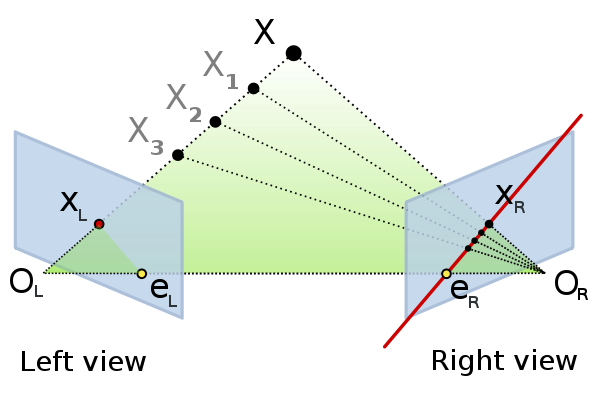
\includegraphics[width=0.6\textwidth]{epipolar_geometry}
\end{figure}

\subsubsection{Piirteiden seuraaminen}
Mönkijän liikuttua noin 75 senttimetrin matkan otetaan toinen kuvapari, jonka kuvien päälle heijastetaan aikaisemmin valitut kiinnostavat piirteet rengasodometrian perusteella. Korrelaatiopohjaisella haulla samat piirteet etsitään uusista kaksiulotteisista kuvista. Nyt uudesta kuvaparista löydetyt halutut piirteet sijoitetaan kolmiulotteiseen malliin edellisen vaiheen tapaan, mutta tällä kertaa sovittaminen on huomattavasti nopeampaa, sillä piirteiden sijainti tiedetään jo edellisen kuvaparin perusteella. Mikäli joidenkin piirteiden sijainti ensimmäisessä kuvaparissa eroaa liikaa toisesta kuvaparista lasketusta sijainnista niin piirteitä ei käytetä enää tulevissa laskuissa.\cite{cheng2005visual}

\subsubsection{Liikkeen luotettava arviointi}
Mikäli rengasodometriasta saatu tieto liikutusta matkasta pitää paikkaansa niin molempien kuvaparien sovittamalla luodussa kolmiulotteisessa mallissa piirteiden sijainnit pysyvät ennaltamäärätyn virhemarginaalin sisällä eikä jatkotoimenpiteitä täten tarvita vaan mönkijä pystyy informaation avulla päivittämään sijaintinsa kartalla. 

Visuaalisesta odometriasta on kuitenkin eniten hyötyä juuri silloin kun muilla tavoin ei voida saada luotettavaa sijainnista kertovaa tietoa. Tämä havaitaan siten, että tunnistettujen piirteiden sijainti eroaa mallissa odotetusta ja eron perusteella määritellään mönkijän todellinen liike kuvaparien ottamisen välissä.

Prosessi on kaksivaiheinen, joista ensimmäisessä luodaan karkea arvio kuvaparien väliselle liikkeelle käyttäen pienimmän neliösumman menetelmää. Tähän löytyy nopea sekä luotettava suljetun muodon ratkaisu. Helpon laskettavuutensa, mutta hitaampia menetelmiä epätarkemman arvion vuoksi ensimmäisellä menetelmällä pyritään ainoastaan poistamaan poikkeavat havainnot, jolloin toinen vaihe voidaan suorittaa nopeammin. Jäljelle jäänyttä joukkoa käytetään toisessa vaiheessa tarkempaan arvioon kuljetun liikeradan laskemiselle. Epätoivotut piirteet poistetaan seuraavalla tavalla:

\begin{enumerate}
\item Valitaan satunnaisesti pieni määrä piirteitä ja lasketaan niiden avulla kuvaparien välinen liike soveltaen pienimmän neliösumman menetelmää.

\item Kaikki aikaisemmissa vaiheissa löydetyt piirteet heijastetaan valittujen pisteiden kanssa samaan kuvaan käyttäen hyväksi ensimmäisessä kohdassa saatua arviota liikeradasta. Jokainen satunnaisesti valittu piirre, joka osuu riittävän lähelle tätä vastaavaa heijastetta saa yhden pisteen.

\item Kahta ensimmäistä vaihetta iteroidaan haluttu määrä ja lopuksi valitaan se piirre, joka on saanut eniten pisteitä. Tätä kolmivaiheista algoritmia voidaan soveltaa kunnes saadaan tarvittava määrä piirteitä, jotka vastasivat karkeaa arviota kuljetusta liikeradasta.
\end{enumerate}

Nyt prosessi on valmis tekemään tarkan arvion käyttäen tilastotieteellistä menetelmää nimeltä suurimman uskottavuuden estimointi. Arvion tekeminen tapahtuu seuraavalla tavalla:

Olkoon $P_pj$ ja $Pcj$ mönkijän sijainti ennen ja jälkeen liikkeen. Jolloin
\[P_{cj} = RP_{pc} + T + e_j,\]
missä $R$ ja $T$ ovat mönkijän rotaatio sekä translaatio ja $e_j$ on yhdistetty virhe piirteiden havaitussa sijainnissa. Tässä arviossa kolme akselin rotaatiota $\theta_R$ ja translaatio T ovat suoraan määritelty minimoimalla eksponenttien summa:
\[\sum r^T_jW_jr_j\]
\[r_j = P_{cj}-RP_{pj}-T,\]
missä $W_j$ on $e_j:n$ kovarianssi-käänteismatriisi. Tämän epälineaarisen ongelman minimointi on toteutettu linearisoimalla sekä iteratiivisella prosessilla. Tarkan algoritmista tekee se, että suurimman uskottavuuden estimoinnissa voidaan eliminoida rotaatiomatriisin arvioinnista syntyvä virhe laskemalla arvio akselien rotaatioille $\theta_R$ suoraan, toisin kuin pienimmän neliösumman menetelmässä. Lisäksi lopullinen arvio pitää sisällään myös tiedon kaikista rengasodometriasta saaduista virheellisistä arvioista, jonka avulla suurimman uskottavuuden estimointi on erittäin tarkka menetelmä sijainnin laskemiseksi.

\cite{cheng2005visual}

\subsection{Algoritmin validointi Maan pinnalla}
Ennen varsinaista käyttöönottoa visuaalista odometriaa kokeiltiin useilla erilaisilla alustoilla kuten esimerkiksi NASAn Jet Propulsion Laboratoryn Rocky 8 -mönkijällä. Kahdella vaarojen havaitsemiseen tarkoitetulla kameraparilla varustettuna laite muistuttaa Marsiin lähetettyjä Spiritiä sekä Opportunityä. Kokeiluun käytetty Johnson Valley tarjoaa mäkisen sekä hienon hiekan vuoksi liukkaan maaperän, jonka tarkoituksena on saada rengasodometria tuottamaan vääriä tuloksia, jolloin konenäön avulla tehdyn paikannuksen hyödyt tulevat esiin. Rockyn todellisen liikkeen sekä asennon mittaamiseen otettiin avuksi takymetri, jonka virhemarginaali pysyy alle kahdessa millimetrissä liikutulla matkalla sekä alle 0.2 asteessa asennon suhteen. Visuaalinen odometria mittasi mönkijän kulkeman matkan reilusti alle tavoitteeksi asetetun 10\% virhemarginaalin ja virhettä kertyi alle 1.5\%. Virhe asennon suhteen pysyi kaikissa testeissä alle viidessä asteessa.

Lähemmäksi Mars-mönkijöiden todellista laitekokoonpanoa päästiin sisätiloissa ajetulla MER Surface System Testbed Lite -järjestelmällä. Ainoa merkittävä ero on lähinnä vaarojen havaitsemiseen tarkoitetussa kameraparissa, jonka kuvissa testimönkijän näkökenttä on 120 astetta verrattuna Mars-mönkijöiden 45 asteeseen. Laitteella ajettiin seitsemän kertaa 35 senttimetrin matka ja visuaalisen odometrian sekä rengasodometrian virheet kirjattiin ylös jokaisella pysähtymiskerralla. Koko matkan ajan konenäkö pystyi pitämään virhemarginaalin alle yhdessä prosentissa, kun taas renkaista saadut mittaukset vaihtelivat luotettavuudessaan, mutta matkan kasvaessa virhemarginaali pääasiassa kasvoi ja ylitti maksimiksi asetetun 10\% arvon. \cite{cheng2005visual}

\subsection{Visuaalinen odometria Marsin pinnalla}
Spirit ja Opportunity kuvaavat ympäristöään näiden mastoihin kiinnitetyillä NAVCAM-kamerapareilla ja kameroiden tuottamat kuvaparit annetaan visuaalisen odometrian käsiteltäväksi. Paras tulos saadaan kun liike tapahtuu kerrallaan enintään 75 senttimetrin askeleissa ja kuvien päällekkäisyys on vähintään 60 prosenttia. Liikkeen aikana rata saa kaareutua maksimissaan 18 astetta. Yhden askeleen vaatima laskenta-aika vaihtelee kahdesta kolmeen minuuttia visuaalisen odometrian ollessa käytössä.

Marsin pinta asettaa toisinaan myös sellaisia haasteita, joissa tämä menetelmä ei tuota hyväksyttävää tulosta. Laajat hiekka-aavikot saattavat sisältää liian vähän konkreettisia piirteitä, jotta niitä olisi tarpeeksi algoritmia varten. Tämän lisäksi edellä mainittujen optimaalisten liikeratojen rikkominen tuotti algoritmille hankaluuksia. Vääriä, mutta mönkijän visuaalisen odometrian oikeaksi mieltämiä ratkaisuja syntyi kahden ajon aikana alkuperäisen konfiguraation takia, jossa kuvista löydettyjen piirteiden ei tarvinnut kattaa riittävän isoa aluetta. Muuttamalla vaadittavasta kattavuudesta kertovaa parametria ongelma korjattiin. Ainoa jatkuvaan tarkkailuun asetettu ongelmakohta ilmeni Opportunity 235:en päivän kohdalla, kun liian piirteetön maasto keskitti visuaalisen odometrian huomion mönkijän omaan varjoon. Tämä tuotti täysin virheellisen tuloksen arvioon kuljetusta matkasta ja tapahtuman jälkeen ohjaajien on täytynyt ottaa mönkijöiden varjot huomioon antaessaan niille käskyn nojautua visuaaliseen odometriaan liikkumisen aikana. 

Visuaalisen odometrian lisäämä autonomisen liikkumisen turvallisuus taas oli yksi selkeistä hyödyistä, joita mönkijöiden päivittäisessä operoinnissa havaittiin. Tämän lisäksi tarkempi liike mahdollisti kehittyneemmän kyvyn tehdä tieteellisiä havaintoja hankalassa maastossa esimerkiksi siten ettei ohjaajien tarvinnut varmistaa mönkijään kiinnitettyjen instrumenttien kohdentamista hitaasti välittyvän näköhavainnon perusteella.

Marsissa viettämästään 394:stä vuorokaudesta Opportunity nojautui visuaaliseen odometriaan 75:nä päivänä. Ajopäiviä mönkijälle kertyi 172, joten algoritmia oli käytössä lähes joka toisena päivänä. Spiritin vastaavat luvut olivat 414 Marsin vuorokautta, joista ajopäiviä oli 184 ja visuaalista odometriaa käytettiin 52:na päivänä. Yhteensä kuvapareja analysoitiin tuona aikana 1 654 kappaletta, joista 1 418 pystyi arvioimaan mönkijän sijainnin sekä asennon riittävän tarkasti. \cite{cheng2005visual}

Huolimatta yllä mainituista ongelmista visuaalinen odometria on yksi mönkijöiden tärkeimmistä työkaluista turvallisen ja itsenäisen liikkumisen toteuttamisessa Marsin pinnalla. Havaituista hyödyistä kertoo myös se, että algoritmi on käytössä vuonna 2011 Marsiin lähetetyssä Curiosity-mönkijässä \cite{grotzinger2012mars}.

\bibliographystyle{alpha}
\bibliography{references-fi}


% --- Appendices ---

% uncomment the following

% \newpage
% \appendix
% 
% \section{Esimerkkiliite}

\end{document}
